\documentclass[./examen.tex]{subfiles}
\begin{document}
\info{Escuela 4-124 Reynaldo Merín  - Evaluación Electrotécnia II}{TEMAS: f.e.m generada por un conductor que se mueve en un campo magnético, Fuerza producida por un conductor que se mueve en un campo magnético, Ley de Faraday-Lenz, regla de la mano izquierda y derecha.}
\begin{center}
\makebox[\textwidth]{Nombre y Apellido:\enspace\hrulefill}
\end{center}
\begin{questions}
 
 \question Un electroimán tiene una superficie de $S=96cm^2$ y su inducción magnética en el hierro es de $B=500Gs$.
 \begin{parts}
    \part[1] Calcular la fuerza de atracción del electroimán $F$ en kilopondios.
 \vspace{2cm}
    \part[1] Calcular la intensidad de campo magnético $H$ si la permeabilidad relativa del núcleo de electroimán es $\mu_r=2000$
  \vspace{2cm}
 \end{parts}
 
\question El anillo cilíndrico de la figura de sección $S=5cm^2$ está construído de chapa magnética $\mu_r=200$, se obtiene un flujo de $\Phi =75000Mx$.  
\begin{parts}
\part[1] Calcular la longitud de la línea media $l_m$ en metros. 
\part[1] Calcular la inducción magnética en el núcleo $B$ en Teslas.
\part[1] Fuerza magnetomotriz $\mathscr{F}$ amperios-vuelta necesarios.
\end{parts}

\begin{figure}[h]
    \centering
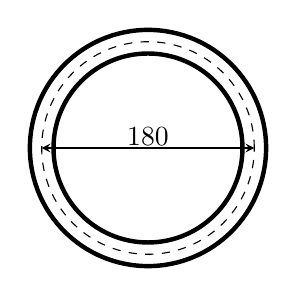
\begin{tikzpicture}[scale=0.015]
    \draw [dashed, thin] (0,0) circle [radius=90];
    \draw [ultra thick] (0,0) circle [radius=100];
    \draw [ultra thick] (0,0) circle [radius=80];
    \draw [stealth-stealth] (-90,0)--(90,0);
    \draw (0,10) node[]{180};
    \end{tikzpicture}
    \end{figure}

\question  Un conductor $l=10cm$ de longitud se mueve dentro de un campo magnético de inducción $B=1400Gs$. 
\begin{parts}
\part[1] Si ejerce sobre el conductor una fuerza de  $F=0,5N$. ¿Qué intensidad $I$ debe circular por un conductor?
\vspace{1cm}
\part[1] Si la corriente fuese de $I=10A$ ¿Cuánta fuerza $F$ se ejerce sobre el conductor en Newtons?
\vspace{1cm}
\end{parts}
  \question Un solenoide de $N=2000$ espiras, longitud de $l=50cm$, $\varnothing=4cm$ y núcleo de madera $\mu_r=1$ el cual tiene arrollado sobre él una bobina de $N=1500$ espiras. 
  \begin{parts}
  \part[2] Calcular la f.e.m. inducida en la bobina cuando se anula en $\Delta t=0,1s$. La corriente es de $I=10A$. 
  \vspace{2cm}
  \end{parts}
  \question[1] Explicar la regla de la mano izquierda, dar 2 ejemplos indicando la dirección de la corriente el campo magnético(inducción) y la dirección de la fuerza.
  \end{questions}
 \end{document}